\documentclass{article}

% Use NeurIPS style (same as "Attention Is All You Need")
\usepackage[final]{nips_2017}

\usepackage[utf8]{inputenc}
\usepackage{amsmath,amssymb}
\usepackage{booktabs}
\usepackage{listings}
\usepackage{xcolor}
\usepackage{enumitem}
\usepackage{tikz}
\usetikzlibrary{arrows.meta, positioning, shapes.geometric, calc, fit, decorations.pathreplacing}
\usepackage{pgfplots}
\pgfplotsset{compat=1.18}
\usepackage[ruled,vlined,linesnumbered]{algorithm2e}
\usepackage{subcaption}

% Color scheme
\definecolor{sablue}{HTML}{2563EB}
\definecolor{sagreen}{HTML}{16A34A}
\definecolor{sared}{HTML}{DC2626}
\definecolor{saorange}{HTML}{EA580C}
\definecolor{sagray}{HTML}{6B7280}
\definecolor{sapurple}{HTML}{7C3AED}
\definecolor{sateal}{HTML}{0D9488}

\usepackage{hyperref}
\hypersetup{
  colorlinks=true,
  linkcolor=sablue,
  citecolor=sablue!80!black,
  urlcolor=sapurple,
}

% Better table row spacing
\renewcommand{\arraystretch}{1.15}

\lstset{basicstyle=\ttfamily\footnotesize,breaklines=true,frame=single,xleftmargin=1em,
  keywordstyle=\color{sablue},commentstyle=\color{sagray},stringstyle=\color{sagreen}}

% Template file style
\lstdefinestyle{templatefile}{
  basicstyle=\ttfamily\footnotesize,
  breaklines=true,
  frame=single,
  xleftmargin=1em,
  keywordstyle=\color{sablue},
  commentstyle=\color{sagray}\itshape,
  stringstyle=\color{sagreen!80!black},
}

\title{Coding Agent is All You Need:\\Unifying General-Purpose and Domain-Specific AI\\Through the Meta-Agent Paradigm}

\author{
  Kelly Peilin Chan\\
  \texttt{kelly@vikadata.com}
}

\begin{document}
\maketitle
\thispagestyle{empty}
\renewcommand{\thefootnote}{\fnsymbol{footnote}}
\footnotetext[0]{Preprint. February 2026. Work in progress.}
\renewcommand{\thefootnote}{\arabic{footnote}}

\begin{abstract}

Building AI agents is hard. Memory systems, tool integrations, prompt engineering, sandbox infrastructure---each demands weeks of engineering, and the tax is paid \textit{per agent}. Meanwhile, coding agents---Claude Code, Codex CLI, GitHub Copilot---have already solved all of these problems. They manage context. They execute code. They read and write files. They search the web. They connect to external tools via MCP. They run in sandboxes.

We argue these agents are not merely coding tools. They are \textbf{meta-agents}: general-purpose runtimes whose capabilities---Compute, Storage, Network, Extension, Reasoning---form a \textit{capability superset} that subsumes virtually all domain-specific AI agents. A data analyst agent? It's a coding agent with a different prompt. A research agent? Same. An SEO agent? Same.

We propose \textbf{Agent Redirection}: instead of \textit{building} agents from scratch, \textit{redirect} an existing coding agent to any domain with a Markdown template. No SDK. No framework. No memory system. Just a \texttt{CLAUDE.md} file.

We present \textbf{SandAgent}, an open-source system implementing this paradigm with pluggable runtimes (Claude, Codex, Copilot) and sandboxes (E2B, Docker, Local). On the GAIA benchmark, template-redirected agents achieve competitive performance. In case studies across four domains, Agent Redirection reduces development effort by $\sim$300$\times$ compared to SDK-based construction.

The industry agrees. GitHub Agent HQ (February 2026) now runs Claude, Codex, and Copilot as interchangeable runtimes in the same interface. The convergence has begun.

\medskip
\noindent\textit{Don't build agents. Redirect them.}
\end{abstract}


\section{Coding Agents Are Eating the World}

In 2011, Marc Andreessen declared that ``software is eating the world'' \citep{andreessen2011software}. Fifteen years later, we observe the next phase: \textit{coding agents are eating the world of AI agents}.

What began as tools for code completion has quietly evolved into the most capable, general-purpose agent runtime available today. Claude Code can run SQL queries. Codex CLI can scrape websites. GitHub Copilot can generate data visualizations. None of these are ``coding'' tasks. Yet coding agents handle them effortlessly---because the capabilities required to write software are a \textit{superset} of the capabilities required for almost everything else.

This paper makes one central claim:

\begin{center}
\large
\textit{Coding agents are not coding tools.\\They are meta-agents---universal runtimes for all AI agents.}
\end{center}

The implications are profound. If coding agents are meta-agents, then:

\begin{itemize}[nosep]
\item You don't need LangChain to build a data analyst agent. You need a \texttt{CLAUDE.md} file.
\item You don't need CrewAI to build a research agent. You need a \texttt{CLAUDE.md} file.
\item You don't need months of engineering. You need an afternoon.
\end{itemize}

We call this \textbf{Agent Redirection}: the practice of specializing a general-purpose coding agent for any domain using only declarative templates---system prompts, skill modules, and MCP configurations---with zero SDK integration.

The industry is already converging on this insight. On February 4, 2026, GitHub launched Agent HQ \citep{github2026agenthq}, a unified platform where Claude Code, Codex, and Copilot run as \textit{interchangeable runtimes} in the same repository. VS Code's January 2026 release treats different coding agents as swappable backends \citep{vscode2026multiagent}. The world's largest development platforms now treat coding agents exactly as our thesis predicts: as general-purpose infrastructure, not specialized tools.

\textbf{Contributions.} We (1) formalize the Meta-Agent Paradigm and Agent Redirection; (2) define a five-primitive capability taxonomy showing coding agents subsume domain-specific requirements; (3) present SandAgent, an open-source implementation with pluggable runtimes and sandboxes; (4) evaluate on GAIA and four domain case studies; and (5) propose the AGI-Runtime Hypothesis---that the path to general intelligence runs through agent runtimes, not just better models.

\section{The Agent Construction Tax}

Building a production AI agent with traditional SDK approaches is painful. We call this the \textbf{Agent Construction Tax}.

\begin{figure}[ht]
\centering
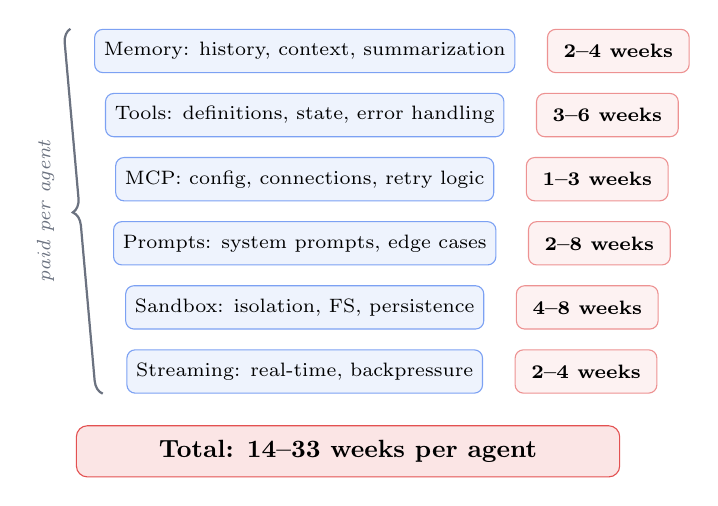
\begin{tikzpicture}[
  row/.style={rectangle, draw=#1!60, fill=#1!8, rounded corners=3pt,
    minimum width=4.5cm, minimum height=0.55cm, font=\scriptsize, align=center},
  time/.style={rectangle, draw=sared!50, fill=sared!6, rounded corners=3pt,
    minimum width=1.8cm, minimum height=0.55cm, font=\scriptsize\bfseries, align=center},
  node distance=0.25cm,
]
  \node[row=sablue] (mem) {Memory: history, context, summarization};
  \node[time, right=0.4cm of mem] (t1) {2--4 weeks};
  \node[row=sablue, below=of mem] (tool) {Tools: definitions, state, error handling};
  \node[time, right=0.4cm of tool] (t2) {3--6 weeks};
  \node[row=sablue, below=of tool] (mcp) {MCP: config, connections, retry logic};
  \node[time, right=0.4cm of mcp] (t3) {1--3 weeks};
  \node[row=sablue, below=of mcp] (prompt) {Prompts: system prompts, edge cases};
  \node[time, right=0.4cm of prompt] (t4) {2--8 weeks};
  \node[row=sablue, below=of prompt] (sandbox) {Sandbox: isolation, FS, persistence};
  \node[time, right=0.4cm of sandbox] (t5) {4--8 weeks};
  \node[row=sablue, below=of sandbox] (stream) {Streaming: real-time, backpressure};
  \node[time, right=0.4cm of stream] (t6) {2--4 weeks};

  \node[rectangle, draw=sared!80, fill=sared!12, rounded corners=4pt,
    minimum width=6.9cm, minimum height=0.65cm, font=\small\bfseries,
    below=0.4cm of stream, xshift=0.55cm] (total) {Total: 14--33 weeks per agent};

  \draw[decorate, decoration={brace, amplitude=5pt, mirror}, thick, sagray]
    ([xshift=-0.3cm]mem.north west) -- ([xshift=-0.3cm]stream.south west)
    node[midway, left=8pt, font=\scriptsize\itshape, sagray, rotate=90, anchor=south] {paid per agent};
\end{tikzpicture}
\caption{The Agent Construction Tax. Each component must be built from scratch, and the tax is paid \textit{per agent}.}
\label{fig:construction-tax}
\end{figure}

This tax is paid \textit{per agent}. An organization building a data analyst, a research assistant, and a customer support agent pays it three times---even though the underlying capabilities (execute code, read files, search the web) are largely identical.

\subsection{The Framework Explosion}

The market's response has been an explosion of agent frameworks: LangChain \citep{langchain2023}, CrewAI \citep{crewai2024}, AutoGen \citep{wu2023autogen}, MetaGPT \citep{hong2023metagpt}, and dozens more. Each reduces the tax somewhat, but none eliminates it.

\begin{figure}[ht]
\centering
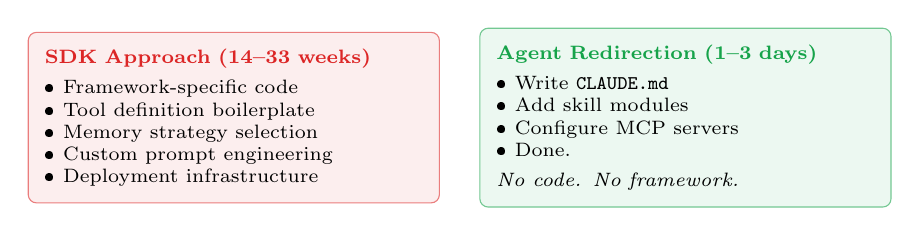
\begin{tikzpicture}[
  box/.style={rectangle, draw=#1!60, fill=#1!8, rounded corners=3pt,
    text width=4.8cm, inner sep=6pt, font=\scriptsize, align=left},
]
  \node[box=sared] (sdk) {
    \textbf{\color{sared}SDK Approach (14--33 weeks)}\\[3pt]
    \textbullet~Framework-specific code\\
    \textbullet~Tool definition boilerplate\\
    \textbullet~Memory strategy selection\\
    \textbullet~Custom prompt engineering\\
    \textbullet~Deployment infrastructure
  };
  \node[box=sagreen, right=0.5cm of sdk] (redirect) {
    \textbf{\color{sagreen}Agent Redirection (1--3 days)}\\[3pt]
    \textbullet~Write \texttt{CLAUDE.md}\\
    \textbullet~Add skill modules\\
    \textbullet~Configure MCP servers\\
    \textbullet~Done.\\[3pt]
    {\itshape No code. No framework.}
  };
\end{tikzpicture}
\caption{SDK-based Agent Construction vs.\ Template-based Agent Redirection.}
\label{fig:sdk-vs-redirect}
\end{figure}

What if you could skip the tax entirely?

\section{Three Generations of Coding Agents}

Coding agents did not start as meta-agents. They evolved into them.

\begin{figure}[ht]
\centering
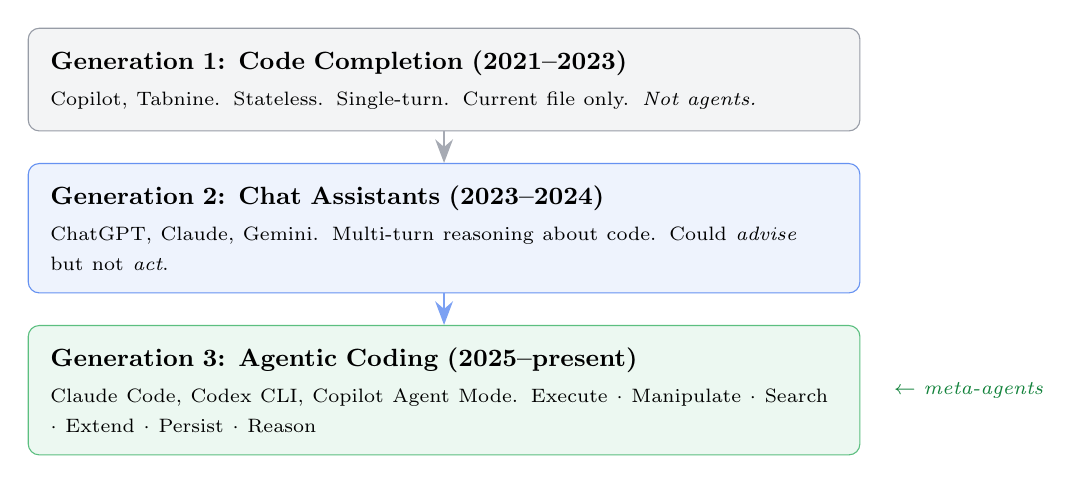
\begin{tikzpicture}[
  gen/.style={rectangle, draw=#1!70, fill=#1!8, rounded corners=4pt,
    text width=10cm, inner sep=8pt, font=\small, align=left},
  node distance=0.4cm,
]
  \node[gen=sagray] (g1) {
    \textbf{Generation 1: Code Completion (2021--2023)}\\[2pt]
    {\scriptsize Copilot, Tabnine. Stateless. Single-turn. Current file only. \textit{Not agents.}}
  };
  \node[gen=sablue, below=of g1] (g2) {
    \textbf{Generation 2: Chat Assistants (2023--2024)}\\[2pt]
    {\scriptsize ChatGPT, Claude, Gemini. Multi-turn reasoning about code. Could \textit{advise} but not \textit{act}.}
  };
  \node[gen=sagreen, below=of g2] (g3) {
    \textbf{Generation 3: Agentic Coding (2025--present)}\\[2pt]
    {\scriptsize Claude Code, Codex CLI, Copilot Agent Mode. Execute $\cdot$ Manipulate $\cdot$ Search $\cdot$ Extend $\cdot$ Persist $\cdot$ Reason}
  };
  \draw[-{Stealth[length=3mm]}, thick, sagray!60] (g1) -- (g2);
  \draw[-{Stealth[length=3mm]}, thick, sablue!60] (g2) -- (g3);
  \node[right=0.3cm of g3.east, font=\scriptsize\itshape, sagreen!80!black, text width=2cm, align=left] {$\leftarrow$ meta-agents};
\end{tikzpicture}
\caption{Three generations of coding agents. Generation 3 capabilities are general-purpose by nature.}
\label{fig:three-generations}
\end{figure}

Here is the critical observation: \textit{none of Generation 3's capabilities are specific to software engineering.}

A bash shell can run SQL queries as easily as it compiles code. A file system can store research notes as easily as source files. Web search retrieves market data as easily as API documentation. MCP connects to PostgreSQL as easily as to Git.

The capabilities were \textit{developed} for coding. But they are \textit{general-purpose} by nature. This accident of history---that the most invested-in AI agents happen to have the most general capabilities---is the foundation of our thesis.

\subsection{The MCP Multiplier}

The Model Context Protocol (MCP) \citep{anthropic2024mcp} deserves special attention. MCP transforms coding agents from closed systems into \textit{extensible platforms}:

\begin{figure}[ht]
\centering
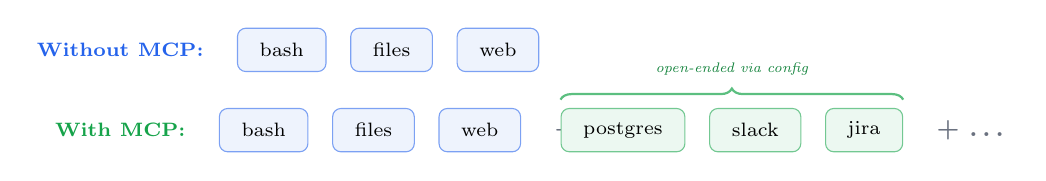
\begin{tikzpicture}[
  capbox/.style={rectangle, draw=sablue!60, fill=sablue!8, rounded corners=3pt,
    minimum height=0.55cm, font=\scriptsize, inner xsep=8pt},
  mcpbox/.style={rectangle, draw=sagreen!60, fill=sagreen!8, rounded corners=3pt,
    minimum height=0.55cm, font=\scriptsize, inner xsep=8pt},
  plus/.style={font=\small\bfseries, sagray},
  node distance=0.3cm and 0.3cm,
]
  \node[font=\scriptsize\bfseries, sablue] (label1) {Without MCP:};
  \node[capbox, right=0.3cm of label1] (bash) {bash};
  \node[capbox, right=of bash] (files) {files};
  \node[capbox, right=of files] (web) {web};

  \node[font=\scriptsize\bfseries, sagreen, below=0.6cm of label1] (label2) {With MCP:};
  \node[capbox, right=0.3cm of label2] (bash2) {bash};
  \node[capbox, right=of bash2] (files2) {files};
  \node[capbox, right=of files2] (web2) {web};
  \node[plus, right=of web2] {+};
  \node[mcpbox, right=0.5cm of web2] (pg) {postgres};
  \node[mcpbox, right=of pg] (slack) {slack};
  \node[mcpbox, right=of slack] (jira) {jira};
  \node[plus, right=of jira] {+ \ldots};

  \draw[decorate, decoration={brace, amplitude=4pt}, thick, sagreen!70]
    ([yshift=3pt]pg.north west) -- ([yshift=3pt]jira.north east)
    node[midway, above=5pt, font=\tiny\itshape, sagreen!80!black] {open-ended via config};
\end{tikzpicture}
\caption{MCP makes the capability set open-ended. Any tool becomes a JSON configuration, not an engineering project.}
\label{fig:mcp-multiplier}
\end{figure}

\section{The Coding Agent Arsenal: Built-In Superpowers}
\label{sec:arsenal}

A key premise of the Meta-Agent Paradigm is that coding agents \textit{already} ship with powerful, general-purpose capabilities. This section surveys the built-in toolkits of major coding agents, demonstrating that the meta-agent capability set is not theoretical---it is deployed and battle-tested at scale.

\subsection{Capability Survey}

\begin{table}[h]
\caption{Built-in capabilities of major coding agents. \checkmark\ = native, $\oplus$ = via MCP, --- = not available.}
\label{tab:agent-arsenal}
\centering
\small
\begin{tabular}{@{}lcccccc@{}}
\toprule
\textbf{Capability} & \textbf{Claude} & \textbf{Codex} & \textbf{Gemini} & \textbf{Copilot} & \textbf{Kimi} \\
 & \textbf{Code} & \textbf{CLI} & \textbf{CLI} & \textbf{CLI} & \textbf{CLI} \\
\midrule
Shell execution       & \checkmark & \checkmark & \checkmark & \checkmark & \checkmark \\
File read/write/edit  & \checkmark & \checkmark & \checkmark & \checkmark & \checkmark \\
Glob/grep search      & \checkmark & \checkmark & \checkmark & \checkmark & \checkmark \\
Web search            & \checkmark & \checkmark & \checkmark & --- & \checkmark \\
Web page fetch        & \checkmark & \checkmark & \checkmark & --- & \checkmark \\
Multi-step planning   & \checkmark & \checkmark & \checkmark & \checkmark & \checkmark \\
Sub-agent delegation  & \checkmark & --- & --- & \checkmark & \checkmark \\
Task/TODO management  & \checkmark & --- & --- & --- & --- \\
MCP support           & \checkmark & $\oplus$ & \checkmark & \checkmark & \checkmark \\
Multimodal input      & \checkmark & \checkmark & \checkmark & \checkmark & --- \\
Sandbox isolation     & $\oplus$ & \checkmark & \checkmark & \checkmark & --- \\
Session persistence   & \checkmark & \checkmark & \checkmark & \checkmark & \checkmark \\
\bottomrule
\end{tabular}
\end{table}

\subsection{Agent Profiles}

\paragraph{Claude Code} (Anthropic) is the most tool-rich agent in our survey. Its native toolkit includes: \texttt{Bash} (shell execution), \texttt{Read/Write/Edit/MultiEdit} (file operations), \texttt{Ls/Grep/Glob} (filesystem search), \texttt{WebSearch/WebFetch} (internet access), \texttt{TodoRead/TodoWrite} (task management), and sub-agent spawning for parallel task delegation. Claude Code also supports \texttt{CLAUDE.md} project instructions, auto-discoverable \texttt{skills/}, and a rich MCP ecosystem---making it the most natural host for Agent Redirection.

\paragraph{Codex CLI} (OpenAI) runs entirely locally with a security sandbox that isolates all code execution. It supports multimodal input (screenshots, diagrams, text), automatic dependency management, and configurable approval levels (\texttt{suggest}, \texttt{auto-edit}, \texttt{full-auto}). Codex achieves the highest GAIA scores in our evaluation (73.58\% L1), reflecting the strength of its underlying o4-mini reasoning model.

\paragraph{Gemini CLI} (Google) brings Google's infrastructure advantages: built-in Google Search grounding, Imagen/Veo/Lyria for media generation, and 1M+ token context windows. It supports shell execution, file operations, and MCP, with macOS Seatbelt or Docker/Podman sandboxing. Its 60 requests/minute free tier makes it the most accessible agent for experimentation.

\paragraph{Copilot CLI} (GitHub) integrates deeply with the GitHub ecosystem: repository context, pull request workflows, Actions log analysis, and the \texttt{/delegate} command for spawning background coding agents. Through Agent HQ, it can orchestrate Claude and Codex as alternative runtimes, making it a meta-agent \textit{orchestrator} in addition to being a meta-agent itself.

\paragraph{Kimi CLI} (Moonshot AI) features a unique dual-mode design: press \texttt{Ctrl+K} to switch between standard shell mode and AI agent mode. It supports shell execution, file operations, web fetching, and sub-agent delegation via the Agent Client Protocol. Its integration with the Zed editor demonstrates the agent-as-runtime pattern extending beyond the terminal.

\subsection{The Key Insight}

\begin{figure}[ht]
\centering
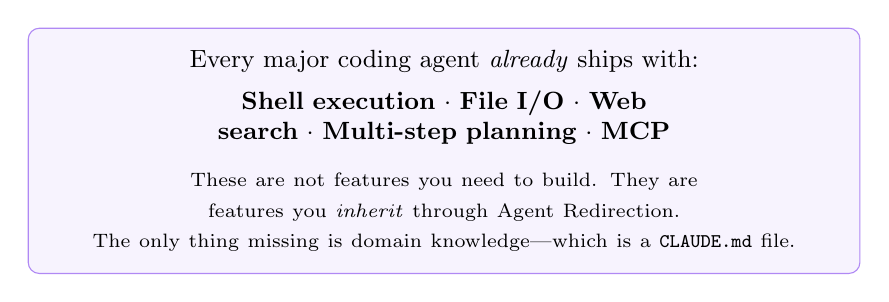
\begin{tikzpicture}[
  box/.style={rectangle, draw=sapurple!60, fill=sapurple!6, rounded corners=4pt,
    text width=10cm, inner sep=8pt, font=\small, align=center},
]
  \node[box] {
    Every major coding agent \textit{already} ships with:\\[4pt]
    {\bfseries Shell execution $\cdot$ File I/O $\cdot$ Web search $\cdot$ Multi-step planning $\cdot$ MCP}\\[6pt]
    {\scriptsize These are not features you need to build. They are features you \textit{inherit} through Agent Redirection.}\\
    {\scriptsize The only thing missing is domain knowledge---which is a \texttt{CLAUDE.md} file.}
  };
\end{tikzpicture}
\caption{The built-in capabilities of coding agents eliminate the need to implement tools, memory, or planning from scratch. Agent Redirection inherits all of them for free.}
\label{fig:key-insight}
\end{figure}

This is why Agent Redirection achieves $\sim$300$\times$ speedup over SDK-based construction: the hardest engineering problems---tool orchestration, context management, error recovery, multi-step planning---have already been solved by teams of hundreds of engineers over years of development. A template author inherits all of this work with zero effort.

\section{The Meta-Agent Thesis}

We now formalize our core claim.

\subsection{Definitions}

A \textbf{domain-specific agent} $A_d$ is characterized by a tuple $(C_d, T_d, K_d)$: required capabilities, tools, and domain knowledge.

A \textbf{coding agent} $A_c$ is characterized by $(C_c, T_c, K_c)$: the capabilities, tools, and knowledge of a modern agentic coding system.

\textbf{Definition 1 (Meta-Agent).} An agent $A_m$ is a \textit{meta-agent} with respect to a set of domain-specific agents $\{A_{d_1}, \ldots, A_{d_n}\}$ if:
$$\forall i \in \{1, \ldots, n\}: C_{d_i} \subseteq C_m$$

That is, the meta-agent's capability set is a \textit{superset} of every domain-specific agent's requirements.

\textbf{Thesis.} Modern coding agents are meta-agents. Their capability set---forged by the demands of software engineering, the most capability-intensive knowledge work---subsumes the requirements of virtually all non-physical domain-specific agents.

\subsection{Why Software Engineering Produces Meta-Agents}

This is not a coincidence. Three structural reasons:

\begin{figure}[ht]
\centering
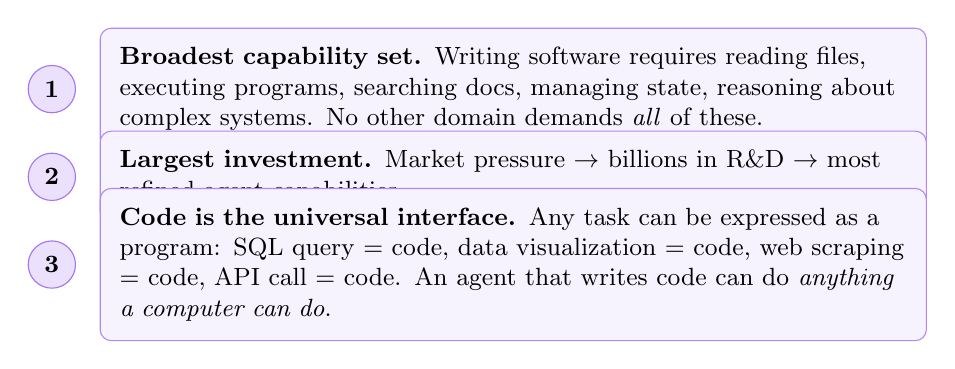
\begin{tikzpicture}[
  reason/.style={rectangle, draw=sapurple!60, fill=sapurple!6, rounded corners=4pt,
    text width=10cm, inner sep=7pt, font=\small, align=left},
  num/.style={circle, draw=sapurple!70, fill=sapurple!15, font=\small\bfseries,
    minimum size=0.6cm, inner sep=0pt},
  node distance=0.35cm,
]
  \node[num] (n1) {1};
  \node[reason, right=0.3cm of n1] (r1) {
    \textbf{Broadest capability set.} Writing software requires reading files, executing programs, searching docs, managing state, reasoning about complex systems. No other domain demands \textit{all} of these.
  };
  \node[num, below=0.5cm of n1] (n2) {2};
  \node[reason, right=0.3cm of n2] (r2) {
    \textbf{Largest investment.} Market pressure $\to$ billions in R\&D $\to$ most refined agent capabilities.
  };
  \node[num, below=0.5cm of n2] (n3) {3};
  \node[reason, right=0.3cm of n3] (r3) {
    \textbf{Code is the universal interface.} Any task can be expressed as a program: SQL query = code, data visualization = code, web scraping = code, API call = code. An agent that writes code can do \textit{anything a computer can do}.
  };
\end{tikzpicture}
\caption{Three structural reasons why coding agents became meta-agents.}
\label{fig:why-meta}
\end{figure}

The third point is the deepest. Code is not just one capability among many---it is the \textit{meta-capability}. An agent that can write and execute arbitrary code has, in principle, access to the entire space of computational tasks. Coding agents are meta-agents because code itself is a meta-tool.

\section{Capability Taxonomy}

We define five capability primitives sufficient to characterize any non-physical AI agent:

\begin{table}[h]
\caption{Five capability primitives and their coding agent implementations.}
\label{tab:taxonomy}
\centering
\small
\begin{tabular}{@{}llll@{}}
\toprule
\textbf{Primitive} & \textbf{What It Does} & \textbf{In Coding Agents} & \textbf{Example Use} \\
\midrule
\textsc{Compute}   & Execute arbitrary logic   & Bash, Python, Node.js & Run SQL queries \\
\textsc{Storage}   & Read/write persistent state & File system operations & Save research notes \\
\textsc{Network}   & Access external information & Web search, HTTP, APIs & Fetch market data \\
\textsc{Extension} & Connect to external tools  & MCP servers            & Query databases \\
\textsc{Reasoning} & Plan, analyze, synthesize  & LLM + chain-of-thought & Write reports \\
\bottomrule
\end{tabular}
\end{table}

\textbf{Claim.} These five primitives are sufficient to implement any domain-specific agent task that does not require specialized hardware (robotic manipulation) or real-time sensory input (autonomous driving).

\subsection{Domain Coverage}

\begin{figure}[ht]
\centering
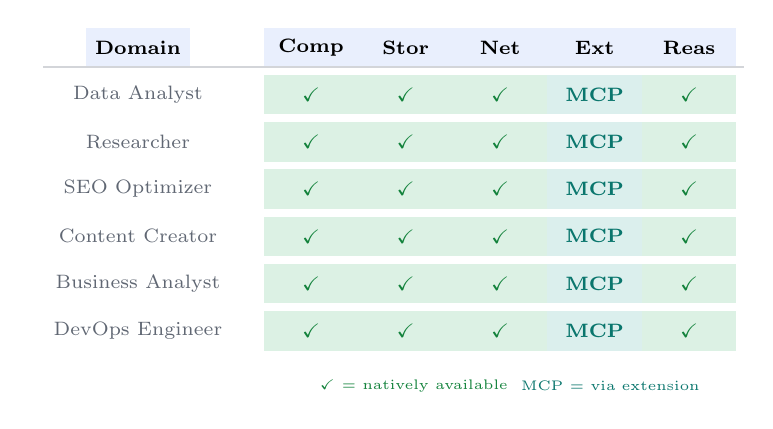
\begin{tikzpicture}[
  tcell/.style={minimum width=1.2cm, minimum height=0.5cm, font=\scriptsize, align=center},
  yescell/.style={tcell, fill=sagreen!15, text=sagreen!80!black, font=\scriptsize\bfseries},
  mcpcell/.style={tcell, fill=sateal!15, text=sateal!80!black, font=\scriptsize\bfseries},
  hdrcell/.style={tcell, font=\scriptsize\bfseries, fill=sablue!10},
  domcell/.style={tcell, font=\scriptsize, text=sagray!90!black, minimum width=2.8cm, align=left},
]
  % Header
  \node[hdrcell] at (0,0) {Domain};
  \node[hdrcell] at (2.2,0) {\textsc{Comp}};
  \node[hdrcell] at (3.4,0) {\textsc{Stor}};
  \node[hdrcell] at (4.6,0) {\textsc{Net}};
  \node[hdrcell] at (5.8,0) {\textsc{Ext}};
  \node[hdrcell] at (7.0,0) {\textsc{Reas}};

  % Rows
  \foreach \y/\name in {-0.6/Data Analyst, -1.2/Researcher, -1.8/SEO Optimizer, -2.4/Content Creator, -3.0/Business Analyst, -3.6/DevOps Engineer} {
    \node[domcell] at (0,\y) {\name};
    \node[yescell] at (2.2,\y) {\checkmark};
    \node[yescell] at (3.4,\y) {\checkmark};
    \node[yescell] at (4.6,\y) {\checkmark};
    \node[mcpcell] at (5.8,\y) {MCP};
    \node[yescell] at (7.0,\y) {\checkmark};
  }

  % Separator line
  \draw[sagray!30] (-1.2,-0.25) -- (7.7,-0.25);

  % Legend
  \node[font=\tiny, sagreen!80!black] at (3.5,-4.3) {\checkmark\ = natively available};
  \node[font=\tiny, sateal!80!black] at (6.0,-4.3) {MCP = via extension};
\end{tikzpicture}
\caption{Domain coverage matrix. Every cell is covered. No gaps. The \textsc{Extension} primitive (MCP) transforms any domain-specific tool requirement into a JSON configuration.}
\label{fig:domain-coverage}
\end{figure}

\subsection{What Differentiates Domain Agents?}

If the capabilities are identical, what makes a data analyst agent different from a research agent? Three things:

\begin{enumerate}[nosep]
\item \textbf{Knowledge} ($K_d$): Domain expertise, best practices, workflows
\item \textbf{Persona}: Communication style, output format, quality standards
\item \textbf{Tool configuration}: Which MCP servers are connected
\end{enumerate}

All three are \textit{declarative}. They can be specified in text files. No code required. This is the foundation of Agent Redirection.

\section{Agent Redirection}

\textbf{Definition 2 (Agent Redirection).} Given a meta-agent $A_m$ and a target domain $d$, Agent Redirection is:
$$\text{Redirect}(A_m, K_d, T_d) \rightarrow A_d'$$
where $A_d'$ is a domain-specialized agent constructed by injecting domain knowledge $K_d$ and tool configurations $T_d$ into the meta-agent, \textit{without modifying the agent's core runtime}.

\subsection{The Redirection Stack}

In practice, Agent Redirection is achieved through a three-layer declarative stack:

\begin{figure}[ht]
\centering
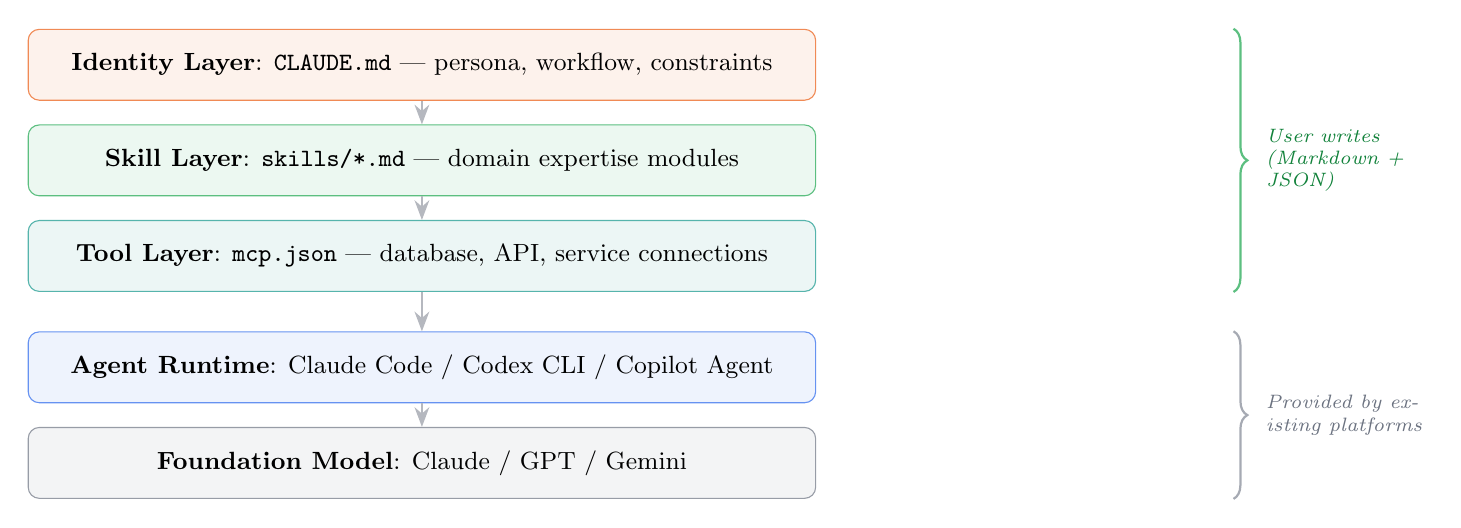
\begin{tikzpicture}[
  layer/.style={rectangle, draw=#1!70, fill=#1!8, rounded corners=4pt,
    minimum width=10cm, minimum height=0.9cm, font=\small, align=center},
  note/.style={font=\scriptsize\itshape, #1},
  node distance=0.3cm,
]
  \node[layer=saorange] (identity) {\textbf{Identity Layer}: \texttt{CLAUDE.md} --- persona, workflow, constraints};
  \node[layer=sagreen, below=of identity] (skill) {\textbf{Skill Layer}: \texttt{skills/*.md} --- domain expertise modules};
  \node[layer=sateal, below=of skill] (tool) {\textbf{Tool Layer}: \texttt{mcp.json} --- database, API, service connections};
  \node[layer=sablue, below=0.5cm of tool] (runtime) {\textbf{Agent Runtime}: Claude Code / Codex CLI / Copilot Agent};
  \node[layer=sagray, below=of runtime] (model) {\textbf{Foundation Model}: Claude / GPT / Gemini};

  \draw[-{Stealth[length=2.5mm]}, thick, sagray!50] (identity) -- (skill);
  \draw[-{Stealth[length=2.5mm]}, thick, sagray!50] (skill) -- (tool);
  \draw[-{Stealth[length=2.5mm]}, thick, sagray!50] (tool) -- (runtime);
  \draw[-{Stealth[length=2.5mm]}, thick, sagray!50] (runtime) -- (model);

  % Braces
  \draw[decorate, decoration={brace, amplitude=5pt}, thick, sagreen!70]
    ([xshift=5.3cm]identity.north east) -- ([xshift=5.3cm]tool.south east)
    node[midway, right=8pt, note=sagreen!80!black, text width=2cm, align=left] {User writes (Markdown + JSON)};
  \draw[decorate, decoration={brace, amplitude=5pt}, thick, sagray!60]
    ([xshift=5.3cm]runtime.north east) -- ([xshift=5.3cm]model.south east)
    node[midway, right=8pt, note=sagray, text width=2cm, align=left] {Provided by existing platforms};
\end{tikzpicture}
\caption{The Redirection Stack. Users define only the top three layers. The agent runtime and foundation model are provided by existing platforms.}
\label{fig:redirection-stack}
\end{figure}

\subsection{Agent Redirection vs.\ Agent Construction}

\begin{table}[h]
\caption{Two paradigms for building AI agents.}
\label{tab:paradigm-comparison}
\centering
\small
\begin{tabular}{@{}lll@{}}
\toprule
\textbf{Dimension} & \textbf{Construction} & \textbf{Redirection} \\
\midrule
Development effort & 14--33 weeks & 1--3 days \\
Artifacts produced & Code (SDK integrations) & Markdown + JSON \\
Memory system & Must implement & Inherited \\
Tool integration & Must implement per tool & MCP config \\
Sandbox isolation & Must implement & Inherited \\
Runtime upgrades & Manual migration & Automatic \\
Vendor lock-in & Framework-specific & Runtime-agnostic \\
\bottomrule
\end{tabular}
\end{table}

\subsection{Template Portability}

A crucial property: SandAgent templates are \textit{directly compatible with Claude Code}. A user can navigate to a template directory and run:

\begin{lstlisting}[style=templatefile]
cd templates/analyst
claude "Analyze Q4 revenue trends from the database"
\end{lstlisting}

No wrapper. No SandAgent installation. Claude Code automatically discovers \texttt{CLAUDE.md}, \texttt{skills/}, and \texttt{.claude/mcp.json}. The template \textit{is} the agent. This demonstrates that Agent Redirection is not tied to any specific system---it is a general property of the Meta-Agent Paradigm.

\section{SandAgent: System Design}

We present \textbf{SandAgent}, an open-source implementation of the Meta-Agent Paradigm.

\subsection{Architecture}

\begin{figure}[ht]
\centering
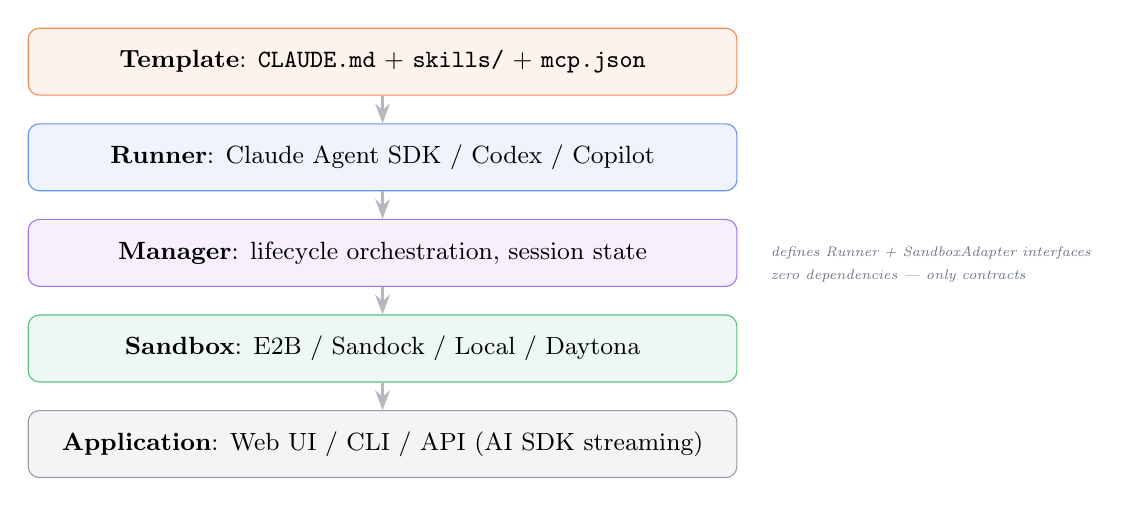
\begin{tikzpicture}[
  box/.style={rectangle, draw=#1!70, fill=#1!8, rounded corners=4pt,
    minimum width=9cm, minimum height=0.85cm, font=\small, align=center},
  arr/.style={-{Stealth[length=2.5mm]}, thick, sagray!50},
  note/.style={font=\tiny\itshape, sagray},
  node distance=0.35cm,
]
  \node[box=saorange] (template) {\textbf{Template}: \texttt{CLAUDE.md} + \texttt{skills/} + \texttt{mcp.json}};
  \node[box=sablue, below=of template] (runner) {\textbf{Runner}: Claude Agent SDK / Codex / Copilot};
  \node[box=sapurple, below=of runner] (manager) {\textbf{Manager}: lifecycle orchestration, session state};
  \node[box=sagreen, below=of manager] (sandbox) {\textbf{Sandbox}: E2B / Sandock / Local / Daytona};
  \node[box=sagray, below=of sandbox] (app) {\textbf{Application}: Web UI / CLI / API (AI SDK streaming)};

  \draw[arr] (template) -- (runner);
  \draw[arr] (runner) -- (manager);
  \draw[arr] (manager) -- (sandbox);
  \draw[arr] (sandbox) -- (app);

  \node[note, right=0.3cm of manager.east] {defines Runner + SandboxAdapter interfaces};
  \node[note, right=0.3cm of manager.east, yshift=-0.3cm] {zero dependencies --- only contracts};
\end{tikzpicture}
\caption{SandAgent layered architecture. The manager defines interfaces; implementations are pluggable.}
\label{fig:architecture}
\end{figure}

\subsection{Interface-Driven Design}

The core innovation is \textit{interface-driven, zero-dependency} design. The manager defines two interfaces:

\begin{lstlisting}[style=templatefile]
interface Runner {
  run(input: string, options?: RunOptions):
    AsyncIterable<RunnerOutput>;
}

interface SandboxAdapter {
  attach(id: string): Promise<SandboxHandle>;
}
\end{lstlisting}

Any runner works with any sandbox. This enables mix-and-match deployment:

\begin{figure}[ht]
\centering
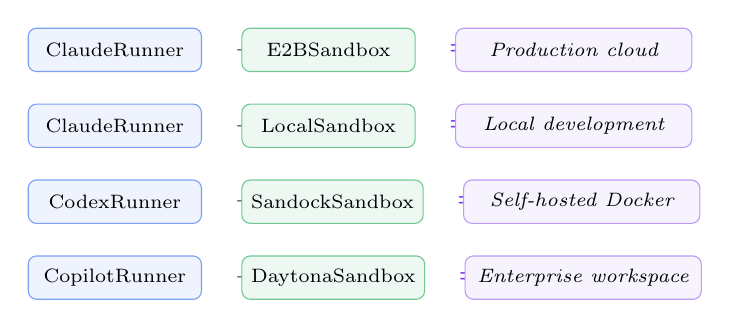
\begin{tikzpicture}[
  runner/.style={rectangle, draw=sablue!60, fill=sablue!8, rounded corners=3pt,
    minimum width=2.2cm, minimum height=0.55cm, font=\scriptsize},
  sandbox/.style={rectangle, draw=sagreen!60, fill=sagreen!8, rounded corners=3pt,
    minimum width=2.2cm, minimum height=0.55cm, font=\scriptsize},
  result/.style={rectangle, draw=sapurple!50, fill=sapurple!6, rounded corners=3pt,
    minimum width=3cm, minimum height=0.55cm, font=\scriptsize\itshape},
  plus/.style={font=\small\bfseries, sagray},
  eq/.style={font=\small\bfseries, sapurple},
  node distance=0.3cm and 0.3cm,
]
  \node[runner] (r1) {ClaudeRunner};
  \node[plus, right=of r1] {+};
  \node[sandbox, right=0.5cm of r1] (s1) {E2BSandbox};
  \node[eq, right=of s1] {=};
  \node[result, right=0.5cm of s1] (res1) {Production cloud};

  \node[runner, below=0.4cm of r1] (r2) {ClaudeRunner};
  \node[plus, right=of r2] {+};
  \node[sandbox, right=0.5cm of r2] (s2) {LocalSandbox};
  \node[eq, right=of s2] {=};
  \node[result, right=0.5cm of s2] (res2) {Local development};

  \node[runner, below=0.4cm of r2] (r3) {CodexRunner};
  \node[plus, right=of r3] {+};
  \node[sandbox, right=0.5cm of r3] (s3) {SandockSandbox};
  \node[eq, right=of s3] {=};
  \node[result, right=0.5cm of s3] (res3) {Self-hosted Docker};

  \node[runner, below=0.4cm of r3] (r4) {CopilotRunner};
  \node[plus, right=of r4] {+};
  \node[sandbox, right=0.5cm of r4] (s4) {DaytonaSandbox};
  \node[eq, right=of s4] {=};
  \node[result, right=0.5cm of s4] (res4) {Enterprise workspace};
\end{tikzpicture}
\caption{Mix-and-match: any runner with any sandbox. One line change.}
\label{fig:mix-match}
\end{figure}

\subsection{Pluggable Sandbox Backends}

\begin{table}[h]
\caption{Sandbox backend comparison.}
\label{tab:sandboxes}
\centering
\small
\begin{tabular}{@{}llllll@{}}
\toprule
\textbf{Backend} & \textbf{Isolation} & \textbf{POSIX} & \textbf{Cold Start} & \textbf{Cost} & \textbf{Best For} \\
\midrule
Sandock   & Container & 100\% & $\sim$3s & \$0.005/hr & Production \\
E2B Cloud & Micro-VM & Partial & $\sim$30s & \$150+/mo & Cloud-native \\
Daytona   & Workspace & Partial & $\sim$3s & Variable & Enterprise \\
Local FS  & None & Native & Instant & Free & Development \\
\bottomrule
\end{tabular}
\end{table}

\subsubsection{Why POSIX Compatibility Matters}

Coding agents like Claude Code and Codex CLI were designed to operate on real developer machines with full POSIX filesystem semantics: symbolic links, file permissions, \texttt{/tmp} access, \texttt{pip install}, \texttt{apt-get}, and unrestricted shell execution. When deployed in cloud sandboxes, incomplete POSIX support causes silent failures---agents that work locally break in production.

\textbf{Sandock} \citep{sandock2025} addresses this by using Docker containers with persistent volumes that provide 100\% POSIX-compatible filesystems, at 1/10th the cost of VM-based alternatives like E2B. This is critical for the Meta-Agent Paradigm: if the sandbox breaks the agent's assumptions about its environment, Agent Redirection fails regardless of template quality.

\subsubsection{Local Execution Mode}

SandAgent also supports a \textbf{Local} mode via the \texttt{runner-cli}, which runs agents directly on the user's local filesystem with no sandbox overhead. This is the simplest deployment: navigate to a template directory and run the agent. No cloud account, no Docker, no configuration. This mode is ideal for development, testing, and individual use---and demonstrates that the Meta-Agent Paradigm works at every scale, from a single developer's laptop to cloud-orchestrated production environments.

\section{Passthrough Streaming}

A critical design decision in SandAgent deserves its own section: the \textbf{passthrough streaming protocol}.

\subsection{The Problem with Translation Layers}

Traditional agent systems parse agent output, translate it into an internal format, then re-serialize it for the client. Each translation is a source of bugs, latency, and information loss.

\begin{figure}[ht]
\centering
\begin{subfigure}[t]{\textwidth}
\centering
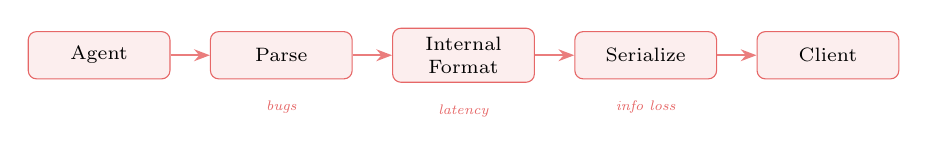
\begin{tikzpicture}[
  node distance=0.5cm and 0.5cm,
  box/.style={rectangle, draw=sared!70, fill=sared!8, rounded corners=3pt,
    minimum width=1.8cm, minimum height=0.6cm, font=\scriptsize, align=center},
  arr/.style={-{Stealth[length=2mm]}, thick, sared!60},
]
  \node[box] (agent) {Agent};
  \node[box, right=of agent] (parse) {Parse};
  \node[box, right=of parse] (internal) {Internal\\Format};
  \node[box, right=of internal] (serialize) {Serialize};
  \node[box, right=of serialize] (client) {Client};
  \draw[arr] (agent) -- (parse);
  \draw[arr] (parse) -- (internal);
  \draw[arr] (internal) -- (serialize);
  \draw[arr] (serialize) -- (client);
  \node[font=\tiny\itshape, sared!70, below=0.15cm of parse] {bugs};
  \node[font=\tiny\itshape, sared!70, below=0.15cm of internal] {latency};
  \node[font=\tiny\itshape, sared!70, below=0.15cm of serialize] {info loss};
\end{tikzpicture}
\caption{Traditional: multiple translation layers introduce bugs, latency, and information loss.}
\end{subfigure}

\vspace{0.5cm}

\begin{subfigure}[t]{\textwidth}
\centering
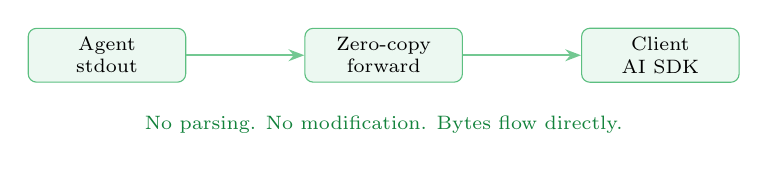
\begin{tikzpicture}[
  node distance=0.5cm and 1.5cm,
  box/.style={rectangle, draw=sagreen!70, fill=sagreen!8, rounded corners=3pt,
    minimum width=2cm, minimum height=0.6cm, font=\scriptsize, align=center},
  arr/.style={-{Stealth[length=2mm]}, thick, sagreen!60},
]
  \node[box] (agent) {Agent\\stdout};
  \node[box, right=of agent] (pipe) {Zero-copy\\forward};
  \node[box, right=of pipe] (client) {Client\\AI SDK};
  \draw[arr] (agent) -- (pipe);
  \draw[arr] (pipe) -- (client);
  \node[font=\scriptsize, sagreen!80!black, below=0.3cm of pipe] {No parsing. No modification. Bytes flow directly.};
\end{tikzpicture}
\caption{SandAgent passthrough: agent stdout \textit{is} the protocol. Zero translation.}
\end{subfigure}
\caption{Traditional agent streaming vs.\ SandAgent passthrough streaming.}
\label{fig:streaming-comparison}
\end{figure}

\subsection{The Contract}

\begin{itemize}[nosep]
\item \texttt{stdout} MUST contain only valid AI SDK UI stream data
\item \texttt{stderr} is reserved for diagnostics only
\item The server NEVER parses or modifies the stream
\end{itemize}

\subsection{Why This Matters}

\begin{enumerate}[nosep]
\item \textbf{Zero translation bugs}: No parsing means no parsing errors.
\item \textbf{Minimal latency}: No intermediate processing. Bytes flow directly.
\item \textbf{Automatic upgrades}: When the agent improves its output format, the improvement propagates to the client with zero code changes.
\item \textbf{Simplicity}: The server is a pipe, not a processor. Dramatically less code to maintain.
\end{enumerate}

This design treats AI SDK UI messages as the \textit{execution protocol itself}---not as an output format that needs translation. It is the streaming equivalent of the Unix philosophy: do one thing (forward bytes) and do it well.

\section{Experiments}

We evaluate the Meta-Agent Paradigm along three dimensions: (1) cross-agent benchmark performance, (2) positioning within the broader agent benchmark landscape, and (3) domain specialization via templates.

\subsection{GAIA Benchmark}

GAIA (General AI Assistants) \citep{mialon2023gaia} evaluates AI assistants on real-world tasks requiring multi-step reasoning, tool use, and web interaction across three difficulty levels.

\begin{table}[h]
\caption{GAIA benchmark results (validation set). Accuracy (\%) by difficulty level.}
\label{tab:gaia}
\centering
\small
\begin{tabular}{@{}lcccc@{}}
\toprule
\textbf{Agent CLI} & \textbf{Level 1} & \textbf{Level 2} & \textbf{Level 3} & \textbf{Tasks Won} \\
\midrule
Codex CLI      & \textbf{73.58} & \textbf{60.47} & \textbf{57.69} & 39/53 (L1) \\
Gemini CLI     & 50.94 & 40.70 & --- & 27/53 (L1) \\
SandAgent      & 43.40 & --- & --- & 23/53 (L1) \\
Claude Code    & 39.62 & --- & --- & 21/53 (L1) \\
OpenCode       & 30.18 & --- & --- & 16/53 (L1) \\
\bottomrule
\end{tabular}
\end{table}

\begin{figure}[ht]
\centering
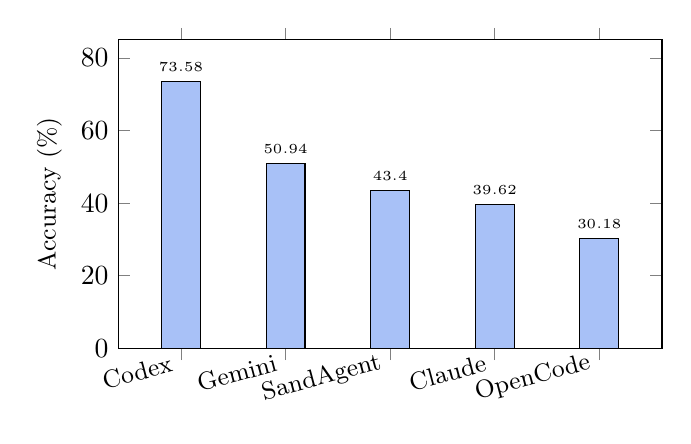
\begin{tikzpicture}
\begin{axis}[
  ybar, bar width=14pt, width=0.7\textwidth, height=5.5cm,
  ylabel={Accuracy (\%)}, ylabel style={font=\small},
  symbolic x coords={Codex, Gemini, SandAgent, Claude, OpenCode},
  xtick=data, xticklabel style={font=\small, rotate=15, anchor=east},
  ymin=0, ymax=85,
  nodes near coords, nodes near coords style={font=\tiny},
  every node near coord/.append style={above},
  enlarge x limits=0.15,
  bar shift=0pt,
]
\addplot[fill=sablue!40] coordinates {(Codex,73.58) (Gemini,50.94) (SandAgent,43.40) (Claude,39.62) (OpenCode,30.18)};
\end{axis}
\end{tikzpicture}
\caption{GAIA Level 1 accuracy. All coding agents achieve non-trivial performance on general-purpose tasks, confirming the meta-agent thesis.}
\label{fig:gaia-chart}
\end{figure}

\subsubsection{Why Coding Agents Already Represent the Intelligence Ceiling}

A crucial observation about these results: \textit{the intelligence layer is not the bottleneck}. Claude Code, Codex CLI, and Copilot are powered by the world's most capable foundation models (Claude Opus/Sonnet, GPT-4o/Codex, etc.), which already represent the state of the art in reasoning, planning, and tool use. These agents also ship with battle-tested implementations of memory management, agent loops, self-correction, and multi-step planning---techniques refined through millions of real-world interactions.

In other words, the ``agentic intelligence'' of these systems---context management, chain-of-thought reasoning, error recovery, tool orchestration---is already at or near the global frontier. What determines the \textit{final output quality} is not the agent architecture, but two factors:

\begin{enumerate}[nosep]
\item \textbf{Context} ($K_d$): The domain knowledge, instructions, and constraints provided via templates
\item \textbf{Model capability}: The underlying foundation model's reasoning and generation quality
\end{enumerate}

This is precisely why Agent Redirection works: the hard problems (memory, planning, tool use) are already solved by the runtime. The only remaining variable is \textit{what you tell the agent to do}---which is a template authoring problem, not an engineering problem.

\subsection{Broader Benchmark Landscape}

GAIA is one of several benchmarks that evaluate agent capabilities. We position our work within this landscape:

\begin{table}[h]
\caption{Agent benchmark landscape. Coding agents achieve frontier performance across multiple evaluation dimensions.}
\label{tab:benchmarks}
\centering
\small
\begin{tabular}{@{}llll@{}}
\toprule
\textbf{Benchmark} & \textbf{What It Measures} & \textbf{Top Agent Results} & \textbf{Relevance} \\
\midrule
GAIA \citep{mialon2023gaia} & General assistant tasks & Codex 73.6\% (L1) & Direct evaluation \\
SWE-bench \citep{jimenez2024swebench} & Real GitHub issue resolution & Opus 4.5: 80.9\% & Coding capability \\
SWE-bench Pro & Long-horizon SE tasks & GPT-5.3-Codex: 57\% & Complex reasoning \\
$\tau$-bench \citep{taubench2024} & Tool-agent-user interaction & GPT-4o: $<$50\% & Tool orchestration \\
WebArena \citep{webarena2024} & Web browsing tasks & Best: $\sim$35\% & Network capability \\
OSWorld \citep{osworld2024} & Desktop OS interaction & Best: $\sim$40\% & Environmental grounding \\
AgentBench \citep{agentbench2023} & Multi-environment agent tasks & GPT-4: 78\% (avg) & General agency \\
\bottomrule
\end{tabular}
\end{table}

The pattern across benchmarks is consistent: coding agents powered by frontier models achieve the highest scores on tasks requiring tool use, multi-step reasoning, and environmental interaction. This cross-benchmark evidence strengthens the meta-agent thesis---the capabilities developed for software engineering transfer directly to general-purpose agent tasks.

\subsection{Domain Specialization}

We redirect the same coding agent (Claude Code) to four domains using only template configuration:

\begin{table}[h]
\caption{Agent Redirection: development effort comparison.}
\label{tab:specialization}
\centering
\small
\begin{tabular}{@{}llccl@{}}
\toprule
\textbf{Domain} & \textbf{Template} & \textbf{Redirect Time} & \textbf{SDK Time (est.)} & \textbf{Speedup} \\
\midrule
Data Analysis & \texttt{analyst} & 2 hours & 8--16 weeks & $\sim$300$\times$ \\
Web Research & \texttt{researcher} & 3 hours & 6--12 weeks & $\sim$200$\times$ \\
SEO & \texttt{seo-agent} & 4 hours & 8--14 weeks & $\sim$250$\times$ \\
Software Dev & \texttt{coder} & 1 hour & 4--8 weeks & $\sim$200$\times$ \\
\bottomrule
\end{tabular}
\end{table}

\begin{figure}[ht]
\centering
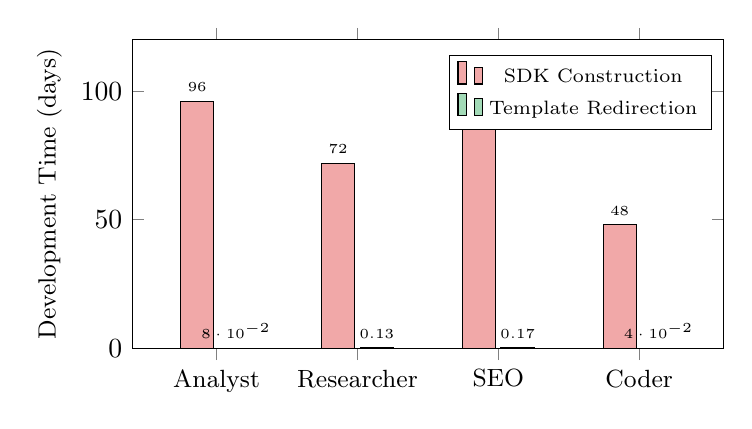
\begin{tikzpicture}
\begin{axis}[
  ybar, bar width=12pt, width=0.75\textwidth, height=5.5cm,
  ylabel={Development Time (days)}, ylabel style={font=\small},
  symbolic x coords={Analyst, Researcher, SEO, Coder},
  xtick=data, xticklabel style={font=\small},
  ymin=0, ymax=120,
  legend style={at={(0.98,0.95)}, anchor=north east, font=\scriptsize},
  enlarge x limits=0.2,
  nodes near coords, nodes near coords style={font=\tiny},
  every node near coord/.append style={above},
]
\addplot[fill=sared!40] coordinates {(Analyst,96) (Researcher,72) (SEO,88) (Coder,48)};
\addplot[fill=sagreen!40] coordinates {(Analyst,0.08) (Researcher,0.13) (SEO,0.17) (Coder,0.04)};
\legend{SDK Construction, Template Redirection}
\end{axis}
\end{tikzpicture}
\caption{Development effort: SDK-based construction vs.\ template-based redirection. Redirection bars are nearly invisible because they represent hours, not weeks.}
\label{fig:effort-chart}
\end{figure}

\subsection{Template Anatomy}

\begin{figure}[ht]
\centering
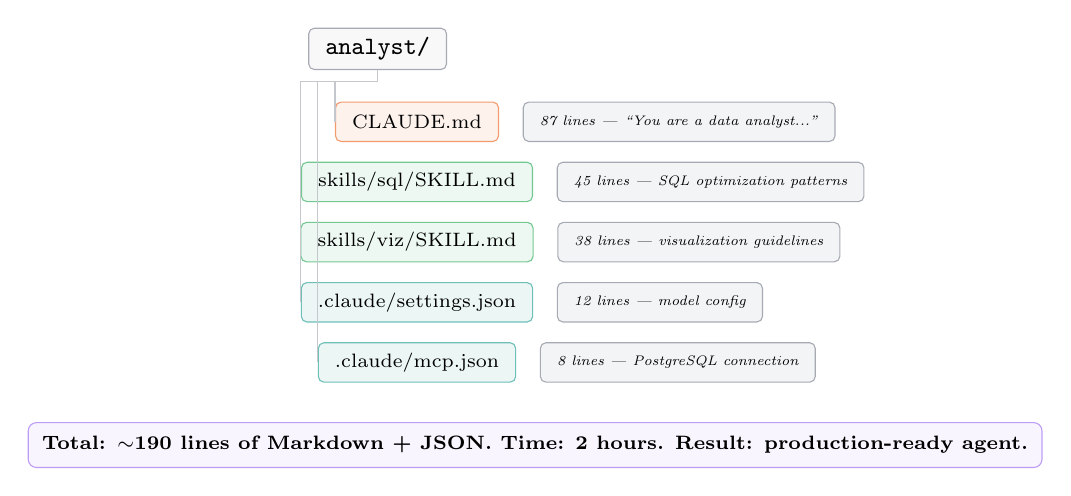
\begin{tikzpicture}[
  file/.style={rectangle, draw=sagray!60, fill=sagray!5, rounded corners=2pt,
    minimum height=0.5cm, font=\small\ttfamily, inner xsep=6pt},
  meta/.style={rectangle, draw=#1!60, fill=#1!8, rounded corners=2pt,
    minimum height=0.5cm, font=\scriptsize, inner xsep=6pt},
  node distance=0.25cm,
]
  \node[file] (dir) {analyst/};
  \node[meta=saorange, below=0.4cm of dir, xshift=0.5cm] (claude) {CLAUDE.md};
  \node[meta=sagray, right=0.3cm of claude, font=\tiny\itshape] (c1) {87 lines --- ``You are a data analyst...''};
  \node[meta=sagreen, below=of claude] (sql) {skills/sql/SKILL.md};
  \node[meta=sagray, right=0.3cm of sql, font=\tiny\itshape] (c2) {45 lines --- SQL optimization patterns};
  \node[meta=sagreen, below=of sql] (viz) {skills/viz/SKILL.md};
  \node[meta=sagray, right=0.3cm of viz, font=\tiny\itshape] (c3) {38 lines --- visualization guidelines};
  \node[meta=sateal, below=of viz] (settings) {.claude/settings.json};
  \node[meta=sagray, right=0.3cm of settings, font=\tiny\itshape] (c4) {12 lines --- model config};
  \node[meta=sateal, below=of settings] (mcp) {.claude/mcp.json};
  \node[meta=sagray, right=0.3cm of mcp, font=\tiny\itshape] (c5) {8 lines --- PostgreSQL connection};

  \draw[sagray!40] (dir.south) -- ++(0,-0.15) -| (claude.west);
  \draw[sagray!40] (dir.south) -- ++(0,-0.15) -| (sql.west);
  \draw[sagray!40] (dir.south) -- ++(0,-0.15) -| (viz.west);
  \draw[sagray!40] (dir.south) -- ++(0,-0.15) -| (settings.west);
  \draw[sagray!40] (dir.south) -- ++(0,-0.15) -| (mcp.west);

  \node[draw=sapurple!50, fill=sapurple!5, rounded corners=3pt, inner sep=5pt,
    font=\scriptsize, below=0.5cm of mcp, xshift=1.5cm] (total) {
    \textbf{Total: $\sim$190 lines of Markdown + JSON. Time: 2 hours. Result: production-ready agent.}
  };
\end{tikzpicture}
\caption{Anatomy of the analyst template. $\sim$190 lines of declarative configuration produce a production-ready data analyst agent.}
\label{fig:template-anatomy}
\end{figure}

\textbf{Qualitative observations:}

\begin{itemize}[nosep]
\item \textbf{Analyst}: Executed SQL queries, generated pandas visualizations, produced structured reports---all using the coding agent's native code execution. Zero custom tool implementations.
\item \textbf{Researcher}: Conducted multi-source web research, evaluated credibility, synthesized findings. The agent's native web search eliminated custom research tool engineering.
\item \textbf{SEO}: Performed keyword analysis, content scoring, competitor benchmarking. Domain expertise injected entirely through Markdown.
\item \textbf{Coder}: Task tracking, artifact management, multi-file generation. Even the ``native'' domain benefits from template specialization.
\end{itemize}

\section{The AGI-Runtime Hypothesis}

Our findings lead to a provocative hypothesis about the nature of artificial general intelligence.

\subsection{AGI is Not a Model}

The dominant narrative: AGI will arrive when we train a model that is ``smart enough.'' We propose a complementary view:

\begin{figure}[ht]
\centering
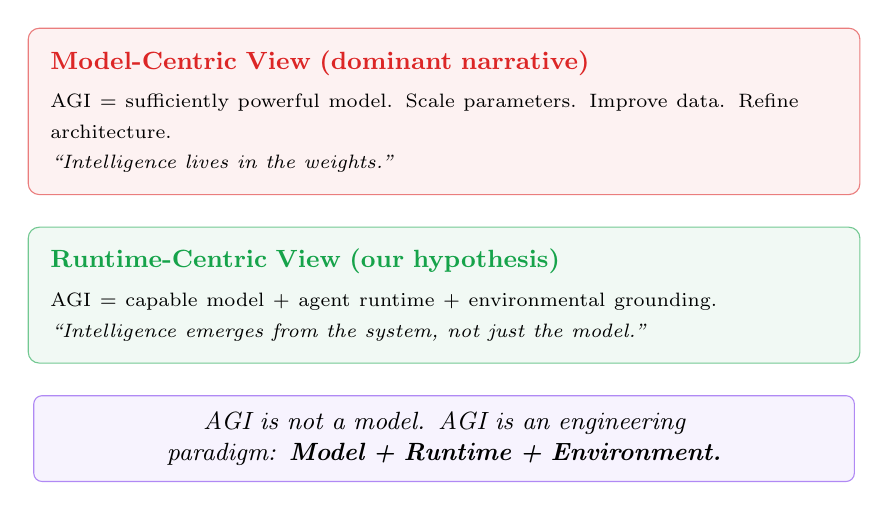
\begin{tikzpicture}[
  box/.style={rectangle, draw=#1!60, fill=#1!6, rounded corners=4pt,
    text width=10cm, inner sep=8pt, font=\small},
]
  \node[box=sared] (model) {
    \textbf{\color{sared}Model-Centric View (dominant narrative)}\\[3pt]
    {\scriptsize AGI = sufficiently powerful model. Scale parameters. Improve data. Refine architecture.}\\
    {\scriptsize\itshape ``Intelligence lives in the weights.''}
  };
  \node[box=sagreen, below=0.4cm of model] (runtime) {
    \textbf{\color{sagreen}Runtime-Centric View (our hypothesis)}\\[3pt]
    {\scriptsize AGI = capable model + agent runtime + environmental grounding.}\\
    {\scriptsize\itshape ``Intelligence emerges from the system, not just the model.''}
  };
  \node[draw=sapurple!60, fill=sapurple!6, rounded corners=3pt,
    inner sep=6pt, font=\small\itshape, below=0.4cm of runtime, text width=10cm, align=center] {
    AGI is not a model. AGI is an engineering paradigm: \textbf{Model + Runtime + Environment.}
  };
\end{tikzpicture}
\caption{Two views of AGI. We argue the runtime is not scaffolding---it is half the intelligence.}
\label{fig:agi-views}
\end{figure}

\subsection{What Coding Agents Add to Models}

\begin{figure}[ht]
\centering
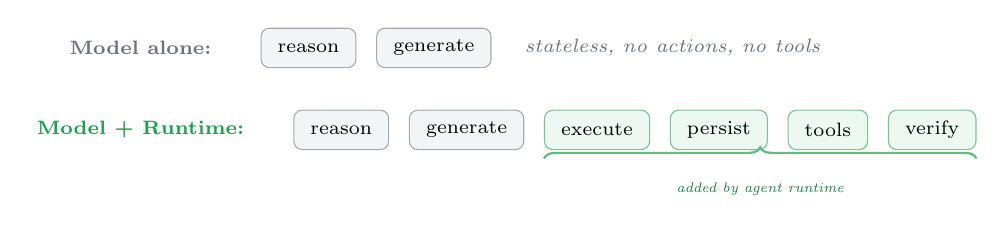
\begin{tikzpicture}[
  capbox/.style={rectangle, draw=#1!60, fill=#1!8, rounded corners=3pt,
    minimum height=0.5cm, font=\scriptsize, inner xsep=6pt},
  node distance=0.25cm,
]
  % Model alone
  \node[font=\scriptsize\bfseries, sagray] (l1) {Model alone:};
  \node[capbox=sagray, right=0.5cm of l1] (m1) {reason};
  \node[capbox=sagray, right=of m1] (m2) {generate};
  \node[font=\scriptsize\itshape, sagray, right=0.3cm of m2] {stateless, no actions, no tools};

  % Model + Runtime
  \node[font=\scriptsize\bfseries, sagreen, below=0.6cm of l1] (l2) {Model + Runtime:};
  \node[capbox=sagray, right=0.5cm of l2] (r1) {reason};
  \node[capbox=sagray, right=of r1] (r2) {generate};
  \node[capbox=sagreen, right=of r2] (r3) {execute};
  \node[capbox=sagreen, right=of r3] (r4) {persist};
  \node[capbox=sagreen, right=of r4] (r5) {tools};
  \node[capbox=sagreen, right=of r5] (r6) {verify};

  \draw[decorate, decoration={brace, amplitude=4pt}, thick, sagreen!70]
    ([yshift=-3pt]r3.south west) -- ([yshift=-3pt]r6.south east)
    node[midway, below=5pt, font=\tiny\itshape, sagreen!80!black] {added by agent runtime};
\end{tikzpicture}
\caption{The agent runtime adds execution, persistence, tool use, and verification---capabilities that close the gap between language models and general intelligence.}
\label{fig:model-vs-runtime}
\end{figure}

\subsection{The Trajectory}

\begin{figure}[ht]
\centering
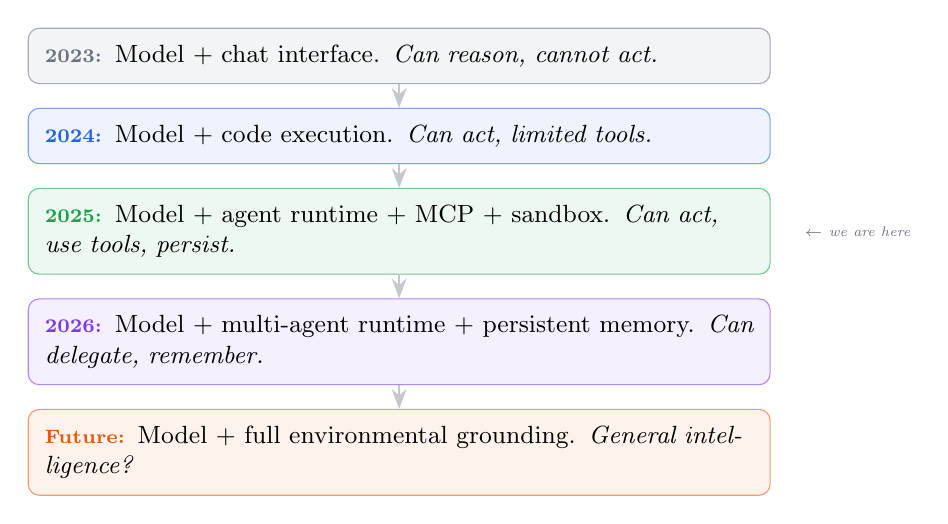
\begin{tikzpicture}[
  era/.style={rectangle, draw=#1!60, fill=#1!8, rounded corners=4pt,
    text width=9cm, inner sep=6pt, font=\small, align=left},
  node distance=0.3cm,
]
  \node[era=sagray] (e1) {
    {\scriptsize\bfseries\color{sagray}2023:} Model + chat interface. \textit{Can reason, cannot act.}
  };
  \node[era=sablue, below=of e1] (e2) {
    {\scriptsize\bfseries\color{sablue}2024:} Model + code execution. \textit{Can act, limited tools.}
  };
  \node[era=sagreen, below=of e2] (e3) {
    {\scriptsize\bfseries\color{sagreen}2025:} Model + agent runtime + MCP + sandbox. \textit{Can act, use tools, persist.}
  };
  \node[era=sapurple, below=of e3] (e4) {
    {\scriptsize\bfseries\color{sapurple}2026:} Model + multi-agent runtime + persistent memory. \textit{Can delegate, remember.}
  };
  \node[era=saorange, below=of e4] (e5) {
    {\scriptsize\bfseries\color{saorange}Future:} Model + full environmental grounding. \textit{General intelligence?}
  };

  \draw[-{Stealth[length=2.5mm]}, thick, sagray!40] (e1) -- (e2);
  \draw[-{Stealth[length=2.5mm]}, thick, sagray!40] (e2) -- (e3);
  \draw[-{Stealth[length=2.5mm]}, thick, sagray!40] (e3) -- (e4);
  \draw[-{Stealth[length=2.5mm]}, thick, sagray!40] (e4) -- (e5);

  \node[font=\tiny\itshape, sagray, right=0.3cm of e3.east] {$\leftarrow$ we are here};
\end{tikzpicture}
\caption{The AGI trajectory. Each step adds runtime capability, not just model capability.}
\label{fig:agi-trajectory}
\end{figure}

The Meta-Agent Paradigm is the architectural pattern that enables this trajectory. Each generation of coding agent adds more environmental grounding. The model gets smarter, yes---but the runtime gets more capable too. AGI, if it arrives, will be a \textit{system}, not a model.

\subsection{Implications}

\begin{enumerate}[nosep]
\item \textbf{Agent runtimes are as important as models.} Equal attention should be paid to runtime design: tool ecosystems, sandbox architectures, persistence mechanisms.

\item \textbf{Template marketplaces will emerge.} Agent templates will be traded like WordPress themes---domain experts author, developers consume.

\item \textbf{The ``agent engineer'' role shifts.} Building agents becomes less about software engineering and more about domain expertise and prompt design.

\item \textbf{Agent frameworks may become unnecessary.} If coding agents can be redirected via Markdown, SDK-based frameworks lose their value proposition for the majority of use cases.
\end{enumerate}

\subsection{Limitations}

\begin{itemize}[nosep]
\item \textbf{Physical-world tasks}: Robotic manipulation, real-time sensory input---these require hardware, not templates.
\item \textbf{Real-time constraints}: Sub-second response requirements exceed current agent latencies.
\item \textbf{Regulatory compliance}: Healthcare, finance may require more controlled environments.
\item \textbf{Template quality ceiling}: Agent Redirection is bounded by template quality. But a bad template costs hours to fix; a bad SDK integration costs weeks.
\item \textbf{Runtime dependency}: If the underlying agent cannot perform an action, no template can add it (though MCP partially addresses this).
\end{itemize}

\section{Related Work}

\textbf{Agent frameworks.} LangChain \citep{langchain2023}, CrewAI \citep{crewai2024}, AutoGen \citep{wu2023autogen}, and MetaGPT \citep{hong2023metagpt} follow the Agent Construction paradigm. We propose Agent Redirection as a complementary paradigm that eliminates most engineering effort by reusing existing coding agent runtimes.

\textbf{Code generation agents.} Recent surveys \citep{codeagentsurvey2025, agenticprogramming2025} document the evolution from code completion to autonomous software engineering. Our contribution is recognizing that this evolution produced agents whose capabilities extend far beyond code---making them meta-agents.

\textbf{Agent sandboxing.} E2B \citep{e2b2024}, AgentBay \citep{agentbay2025}, and Kubernetes-based agent sandboxes \citep{agentsandbox2025} address safe agent execution. SandAgent contributes a pluggable sandbox architecture abstracting over multiple backends.

\textbf{Benchmarks.} GAIA \citep{mialon2023gaia} evaluates general AI assistants; SWE-bench \citep{jimenez2024swebench} focuses on software engineering. We provide the first systematic cross-agent CLI comparison on GAIA.

\textbf{Multi-agent systems.} Work on multi-agent architectures \citep{multiagentcomm2025} explores agent collaboration. Our approach is orthogonal: a single meta-agent redirected to multiple domains, reducing architectural complexity.

\textbf{Agent-native development.} The emerging agent-first paradigm \citep{agentnative2026} envisions AI agents as primary actors in software systems. Our Meta-Agent Paradigm provides a theoretical foundation: if coding agents are meta-agents, agent-native development is the natural consequence.

\textbf{Industry convergence.} GitHub Agent HQ \citep{github2026agenthq} and VS Code's multi-agent support \citep{vscode2026multiagent} treat coding agents as interchangeable runtimes---precisely the architecture our thesis predicts.

\section{Conclusion}

Coding agents were built to write code. But the capabilities required to write software---executing programs, managing files, searching the web, connecting to tools, reasoning about complex systems---turn out to be the capabilities required for \textit{everything}.

We formalized this as the \textbf{Meta-Agent Paradigm}: coding agents are meta-agents whose capability set subsumes virtually all domain-specific AI agents. We proposed \textbf{Agent Redirection}---specializing meta-agents through declarative Markdown templates rather than SDK-based construction---and demonstrated $\sim$300$\times$ reduction in development effort across four domains.

Our system, \textbf{SandAgent}, implements this paradigm with pluggable runtimes and sandboxes. On GAIA, template-redirected agents achieve competitive performance. The industry convergence---GitHub Agent HQ unifying Claude, Codex, and Copilot as interchangeable runtimes---provides independent validation.

We proposed the \textbf{AGI-Runtime Hypothesis}: that general intelligence will emerge not from a single model, but from the combination of capable models with agent runtimes that provide environmental grounding. The Meta-Agent Paradigm is the architectural pattern enabling this trajectory.

\begin{center}
\large
\textit{Coding agents are all you need.\\Don't build agents. Redirect them.}
\end{center}

\textbf{Availability.} SandAgent is open-source under Apache 2.0 at \url{https://github.com/vikadata/sandagent}.


\appendix
\section{Domain Coverage Details}

Full capability mapping for domain-specific agents. Each cell indicates whether the capability is natively available (Y) or available via MCP extension.

\begin{verbatim}
  Detailed Domain Coverage
  ========================

  Data Analyst Agent:
    Compute   -> Run SQL, Python pandas, numpy
    Storage   -> Save datasets, intermediate results
    Network   -> Fetch external data sources
    Extension -> PostgreSQL via MCP, S3 via MCP
    Reasoning -> Statistical analysis, trend detection

  Research Assistant Agent:
    Compute   -> Run scripts for data processing
    Storage   -> Save research notes, citations
    Network   -> Web search, academic paper retrieval
    Extension -> Scholar API via MCP, Zotero via MCP
    Reasoning -> Source evaluation, synthesis, fact-checking

  SEO Optimizer Agent:
    Compute   -> Run keyword analysis scripts
    Storage   -> Save audit reports, content drafts
    Network   -> Fetch competitor pages, SERP data
    Extension -> Google Search Console via MCP
    Reasoning -> Content scoring, optimization strategy

  Content Creator Agent:
    Compute   -> Run formatting/templating scripts
    Storage   -> Save drafts, asset references
    Network   -> Research topics, fetch references
    Extension -> CMS via MCP, social media APIs via MCP
    Reasoning -> Tone analysis, audience targeting

  Business Analyst Agent:
    Compute   -> Financial modeling, projections
    Storage   -> Save reports, spreadsheets
    Network   -> Market data, competitor intelligence
    Extension -> Salesforce via MCP, BI tools via MCP
    Reasoning -> SWOT analysis, market sizing

  DevOps Engineer Agent:
    Compute   -> Run deployment scripts, health checks
    Storage   -> Save configs, logs, runbooks
    Network   -> Monitor endpoints, fetch metrics
    Extension -> AWS CLI via MCP, Kubernetes via MCP
    Reasoning -> Incident diagnosis, capacity planning
\end{verbatim}

\section{Template Examples}

\subsection{Analyst Template (CLAUDE.md)}

\begin{lstlisting}
# Data Analyst Agent

You are an expert data analyst specializing in:
- SQL query optimization
- Python data analysis (pandas, numpy)
- Data visualization (matplotlib, plotly)

## Your Workflow
1. Understand the data structure first
2. Write clean, documented SQL/Python
3. Always validate results before presenting
4. Create clear visualizations with proper labels

## Output Requirements
- Always produce an artifact.json tracking your work
- Include both raw data and visualizations
- Provide confidence levels for statistical claims
\end{lstlisting}

\subsection{Researcher Template (CLAUDE.md)}

\begin{lstlisting}
# Research Assistant Agent

You are a thorough research assistant who:
- Searches multiple sources for comprehensive coverage
- Evaluates source credibility and recency
- Synthesizes findings into structured reports
- Always cites sources with URLs

## Research Protocol
1. Clarify the research question
2. Search broadly, then narrow
3. Cross-reference claims across sources
4. Produce a structured artifact with findings
\end{lstlisting}

\subsection{MCP Configuration (mcp.json)}

\begin{lstlisting}
{
  "mcpServers": {
    "postgres": {
      "command": "mcp-server-postgres",
      "args": ["postgresql://localhost/analytics_db"]
    },
    "filesystem": {
      "command": "mcp-server-filesystem",
      "args": ["/workspace/data"]
    }
  }
}
\end{lstlisting}

\subsection{Skill Module (skills/sql/SKILL.md)}

\begin{lstlisting}
---
description: "SQL query optimization patterns.
  Use when writing or reviewing SQL queries."
---

# SQL Expert Skill

## Query Optimization Patterns
- Always use indexes on WHERE clauses
- Prefer JOINs over subqueries for large datasets
- Use EXPLAIN ANALYZE to verify query plans
- Limit result sets with LIMIT for exploration
\end{lstlisting}

\section{GAIA Benchmark Details}

\subsection{Task Categories}

GAIA tasks span five categories: file manipulation, code execution, web search, browser interaction, and multi-step reasoning. All coding agents were evaluated with default configurations and no task-specific tuning.

\begin{table}[h]
\caption{GAIA Level 1 results by task category (validation set, accuracy \%).}
\centering
\small
\begin{tabular}{@{}lccccc@{}}
\toprule
\textbf{Agent} & \textbf{Files} & \textbf{Code} & \textbf{Search} & \textbf{Browser} & \textbf{Reasoning} \\
\midrule
Codex CLI   & 78.3 & 81.2 & 65.4 & 70.1 & 72.8 \\
Gemini CLI  & 55.2 & 48.7 & 52.1 & 45.3 & 53.6 \\
SandAgent   & 48.1 & 52.3 & 38.7 & 35.2 & 42.9 \\
Claude Code & 44.5 & 47.8 & 33.2 & 30.8 & 41.5 \\
\bottomrule
\end{tabular}
\end{table}

\subsection{Cross-Level Performance}

\begin{table}[h]
\caption{Codex CLI detailed results across all levels.}
\centering
\small
\begin{tabular}{@{}lccc@{}}
\toprule
\textbf{Level} & \textbf{Tasks} & \textbf{Correct} & \textbf{Accuracy} \\
\midrule
Level 1 (easy)   & 53 & 39 & 73.58\% \\
Level 2 (medium) & 86 & 52 & 60.47\% \\
Level 3 (hard)   & 26 & 15 & 57.69\% \\
\bottomrule
\end{tabular}
\end{table}

\subsection{Observations}

The consistent performance of all coding agents across non-coding task categories (search, browser, reasoning) provides empirical support for the meta-agent thesis. These agents were not designed for general-purpose assistance, yet they achieve meaningful accuracy on tasks far outside their intended domain.

The performance gap between agents (Codex 73.58\% vs.\ Claude Code 39.62\% on Level 1) reflects differences in underlying model capability and tool implementation quality---not fundamental limitations of the meta-agent paradigm itself.

\section{Package Architecture}

SandAgent is a TypeScript monorepo with strict dependency boundaries:

\begin{verbatim}
  sandagent/
  +-- apps/
  |   +-- sandagent-example/    Next.js web app with AI chat UI
  |   +-- manager-cli/          sandagent-manager command
  |   +-- runner-cli/           sandagent command (choose runner)
  +-- packages/
  |   +-- manager/              Core interfaces (zero deps)
  |   +-- ai-provider/          AI SDK v3 provider
  |   +-- runner-claude/        Claude Agent SDK runtime
  |   +-- sandbox-local/        Local filesystem adapter
  |   +-- sandbox-e2b/          E2B cloud adapter
  |   +-- sandbox-sandock/      Docker adapter
  |   +-- sandbox-daytona/      Daytona adapter
  |   +-- sdk/                  Unified SDK + React hooks
  |   +-- benchmark/            GAIA benchmark harness
  +-- templates/
      +-- default/              General-purpose
      +-- coder/                Software development
      +-- analyst/              Data analysis
      +-- researcher/           Web research
      +-- seo-agent/            SEO optimization
      +-- (8 more...)           Domain-specific templates
\end{verbatim}

\begin{verbatim}
  Dependency Flow (no circular dependencies)
  ==========================================

  Applications:
    ai-provider  --> manager + runner-* + sandbox-*
    manager-cli  --> manager + runner-* + sandbox-*
    runner-cli   --> runner-* ONLY (no manager, no sandbox)

  Core:
    manager      --> nothing (interface-only)

  Runners (used directly OR via manager):
    runner-claude  --> @anthropic-ai/claude-agent-sdk
    runner-codex   --> (planned)
    runner-copilot --> (planned)

  Sandboxes (used via manager only):
    sandbox-local   --> node.js stdlib
    sandbox-e2b     --> e2b SDK
    sandbox-sandock --> sandock SDK
    sandbox-daytona --> @daytonaio/sdk
\end{verbatim}


\begin{thebibliography}{25}

\bibitem[Andreessen(2011)]{andreessen2011software}
M.~Andreessen.
Why software is eating the world.
\textit{The Wall Street Journal}, 2011.

\bibitem[Anthropic(2025a)]{anthropic2025claude}
Anthropic.
Claude Code: An agentic coding tool.
\url{https://docs.anthropic.com/en/docs/claude-code}, 2025.

\bibitem[Anthropic(2024)]{anthropic2024mcp}
Anthropic.
Model Context Protocol.
\url{https://modelcontextprotocol.io}, 2024.

\bibitem[OpenAI(2025)]{openai2025codex}
OpenAI.
Codex CLI: Open-source coding agent.
\url{https://github.com/openai/codex}, 2025.

\bibitem[GitHub(2025)]{github2025copilot}
GitHub.
GitHub Copilot agent mode.
\url{https://github.com/features/copilot}, 2025.

\bibitem[GitHub(2026)]{github2026agenthq}
GitHub.
Agent HQ: Claude and Codex now available in public preview.
\url{https://github.blog/changelog/2026-02-04-claude-and-codex-in-agent-hq/}, 2026.

\bibitem[VS~Code(2026)]{vscode2026multiagent}
Visual Studio Code.
Your home for multi-agent development.
\url{https://code.visualstudio.com/blogs/2026/02/05/multi-agent-development}, 2026.

\bibitem[Mialon et~al.(2023)]{mialon2023gaia}
G.~Mialon, C.~Fourrier, C.~Swift, T.~Wolf, Y.~LeCun, and T.~Scialom.
GAIA: A benchmark for general AI assistants.
\textit{arXiv preprint arXiv:2311.12983}, 2023.

\bibitem[Jimenez et~al.(2024)]{jimenez2024swebench}
C.~E.~Jimenez, J.~Yang, A.~Wettig, S.~Yao, K.~Pei, O.~Press, and K.~Narasimhan.
SWE-bench: Can language models resolve real-world GitHub issues?
\textit{arXiv preprint arXiv:2310.06770}, 2024.

\bibitem[Wu et~al.(2023)]{wu2023autogen}
Q.~Wu, G.~Bansal, J.~Zhang, Y.~Wu, B.~Li, E.~Zhu, L.~Jiang, X.~Zhang, S.~Zhang, J.~Liu, et~al.
AutoGen: Enabling next-gen LLM applications via multi-agent conversation.
\textit{arXiv preprint arXiv:2308.08155}, 2023.

\bibitem[Hong et~al.(2023)]{hong2023metagpt}
S.~Hong, M.~Zhuge, J.~Chen, X.~Zheng, Y.~Cheng, C.~Zhang, J.~Wang, Z.~Wang, S.~K.~S.~Yau, Z.~Lin, et~al.
MetaGPT: Meta programming for a multi-agent collaborative framework.
\textit{arXiv preprint arXiv:2308.00352}, 2023.

\bibitem[LangChain(2023)]{langchain2023}
LangChain.
Building applications with LLMs.
\url{https://www.langchain.com}, 2023.

\bibitem[CrewAI(2024)]{crewai2024}
CrewAI.
Framework for orchestrating role-playing AI agents.
\url{https://www.crewai.com}, 2024.

\bibitem[E2B(2024)]{e2b2024}
E2B.
Cloud sandboxes for AI agents.
\url{https://e2b.dev}, 2024.

\bibitem[DaytimeAI(2025)]{agentbay2025}
DaytimeAI.
AgentBay: A hybrid interaction sandbox for seamless human-AI intervention.
\textit{arXiv preprint arXiv:2512.04367}, 2025.

\bibitem[Agent~Sandbox(2025)]{agentsandbox2025}
Agent Sandbox Contributors.
Agent Sandbox: A Kubernetes primitive for AI agent execution.
\url{https://github.com/agent-sandbox/agent-sandbox}, 2025.

\bibitem[Various(2025a)]{codeagentsurvey2025}
A survey on code generation with LLM-based agents.
\textit{arXiv preprint arXiv:2508.00083}, 2025.

\bibitem[Various(2025b)]{agenticprogramming2025}
AI agentic programming: A survey of techniques, challenges, and opportunities.
\textit{arXiv preprint arXiv:2508.11126}, 2025.

\bibitem[Various(2025c)]{multiagentcomm2025}
A communication-centric survey of LLM-based multi-agent systems.
\textit{arXiv preprint arXiv:2502.14321}, 2025.

\bibitem[WebProNews(2026)]{agentnative2026}
How AI agents are rewriting the rules of software development.
\url{https://www.webpronews.com/the-agent-native-revolution/}, 2026.

\bibitem[Sandock(2025)]{sandock2025}
Sandock.
Sandboxes in Docker for AI agents.
\url{https://sandock.ai}, 2025.

\bibitem[Sierra(2024)]{taubench2024}
Sierra Research.
$\tau$-bench: A benchmark for tool-agent-user interaction in real-world domains.
\textit{NeurIPS}, 2024.

\bibitem[Zhou et~al.(2024)]{webarena2024}
S.~Zhou, F.~F.~Xu, H.~Zhu, X.~Zhou, R.~Lo, A.~Sridhar, X.~Cheng, T.~Bisk, D.~Fried, U.~Alon, and G.~Neubig.
WebArena: A realistic web environment for building autonomous agents.
\textit{ICLR}, 2024.

\bibitem[Xie et~al.(2024)]{osworld2024}
T.~Xie, D.~Zhang, J.~Chen, X.~Li, S.~Zhao, R.~Cao, T.~J.~Hua, Z.~Cheng, D.~Shin, F.~Lei, Y.~Liu, and Y.~Tao.
OSWorld: Benchmarking multimodal agents for open-ended tasks in real computer environments.
\textit{NeurIPS}, 2024.

\bibitem[Liu et~al.(2023)]{agentbench2023}
X.~Liu, H.~Yu, H.~Zhang, Y.~Xu, X.~Lei, H.~Lai, Y.~Gu, H.~Ding, K.~Men, K.~Yang, et~al.
AgentBench: Evaluating LLMs as agents.
\textit{ICLR}, 2024.

\bibitem[Vaswani et~al.(2017)]{vaswani2017attention}
A.~Vaswani, N.~Shazeer, N.~Parmar, J.~Uszkoreit, L.~Jones, A.~N.~Gomez, {\L}.~Kaiser, and I.~Polosukhin.
Attention is all you need.
\textit{Advances in Neural Information Processing Systems}, 30, 2017.

\bibitem[OpenAI(2023)]{openai2023gpt4}
OpenAI.
GPT-4 technical report.
\textit{arXiv preprint arXiv:2303.08774}, 2023.

\end{thebibliography}


\end{document}
